\chapter{Topology improvements}
\label{c:topology}

In 2D, dislocations are parametrised as points on a surface. Therefore aside from annihilation, interactions with grain boundaries \cite{grain_size_eff1, grain_size_eff2}, and perhaps the creation of superdislocations, topological changes in the dislocation network can be mostly ignored. However, in 3D, dislocations are parametrised as lines in a volume. This gives rise to extra complexities that result from multiple dislocations coming into contact with one another. These reactions ultimately lead to the formation of many secondary structures with their own properties that affect the rest of the network.

The local dislocation density at these interaction sites, particularly arround sessile (immobile) junctions, tends to increase with time. Therefore so do the local stress gradients, and with increasing stress gradients come increasing velocity gradients, which lead to global decreases in timestep. But a smaller timestep is not the only consequence, increases in dislocation density also mean higher probabilities of dislocation-dislocation interactions, so the phenomenon is autocatalytic and self-perpetuating. So properly accounting for these changes is of the utmost importance, particularly for simulations with high dislocation densities such as nanoindentation. This chapter details these improvements.

\section{Collision}\label{s:collision}

\subsection{Hinges}\label{ss:hinges}
The lowest hanging fruit and most obvious problem were collisions that share a lot of similarities with the remeshing criteria that checks for a minimum area enclosed between two segments connected by a single node, as shown in \cref{f:hinge}. A single dislocation hinge can lead to three different final topologies, the conditions for which can be simultaneously met in any combination
\begin{enumerate}
    \item Remeshing to eliminate the middle node because the area, $a$, enclosed by the triangle created by segments $s_1$ and $s_2$ is less than the minimum allowable area, $a_{\rvar{min}}$.
    \item Colliding $s_1$ into $s_2$ if the minimum distance between the non-hinge node of $s_1$ (the node $s_1$ does not share with $s_2$) and segment $s_2$ is less than the collision distance, $l_{\rvar{col}}$.
    \item Colliding $s_2$ into $s_1$ if the minimum distance between the non-hinge node of $s_2$ and segment $s_1$ is less than the collision distance, $l_{\rvar{col}}$.
\end{enumerate}
\begin{figure}
    \centering
    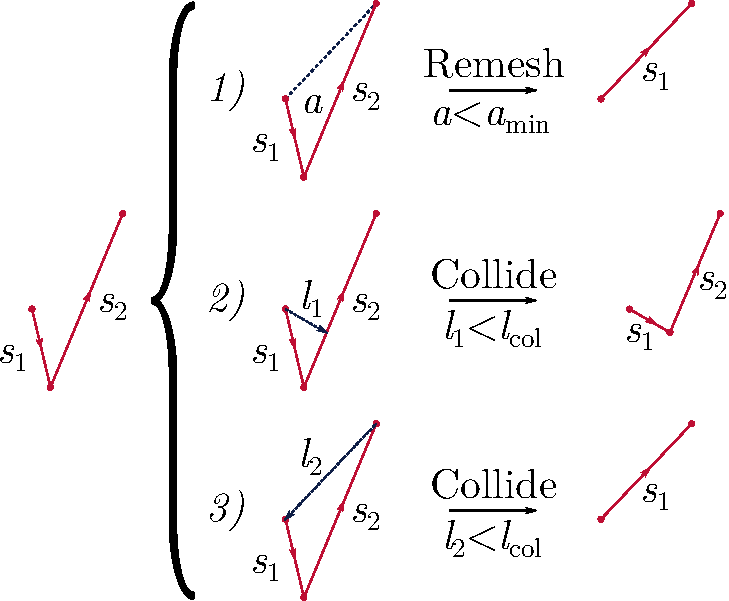
\includegraphics[width=0.5\linewidth]{hinge.pdf}
    \caption[A single dislocation hinge can lead to three different final topologies.]{A single dislocation hinge can lead to three different final topologies, the conditions for which can be simultaneously met in any combination.}
    \label{f:hinge}
\end{figure}

The combination in which these conditions can be met, and the order in which they are checked will have drastic downstream consequences (see \cref{s:nonCommutativity}). \emph{Especially} at high dislocation densities where multiple collisions happen at every timestep. This had not been an issue in prior to fixing the integrator and matrix inversion, but simulations could now advance to a point where this was having a significant impact, particularly in Haiyang Yu's nanoindentation simulations.

This was a multi-stage fix, where each fix progressively uncovered more and more shortcomings resulting from the unavoidable coupling between topological operations. These progressive fixes are detailed in \cref{s:nonCommutativity,s:remeshing}. Here we will only focus on problems with collisions.

The first fix involved prioritising hinge collisions above others, which we call two-line collisions. This meant detecting and forming the new connection. The rationale for this is that a segments in a hinge are close enough to and connected with each other at a node already that they will interact more strongly than two unconnected segments approaching one another.

The second was much more subtle. \Cref{f:hinge} has two options for colliding a hinge. And they both result in differently sized segments $l_1 < l_2$. The one the code calculated depended on which segment, $s_1$ or $s_2$ it came across. If $s_1$ was first, then the answer would be $l_1$, otherwise it would be $l_2$. At the very least, the answer should be the same for a given network regardless of how it is represented. So the first step is to ensure one of these is always chosen, but once this is done it is a simple case of calculating the distance from the short segment to the long one.

Remeshing used to be called after finding a \emph{single} collision. This worked well when the number of collisions at a given time step was small. The problems with this are detailed in \cref{s:nonCommutativity}. But before moving on to that, it became apparent that there was another issue with the collision detection.

\subsection{Collision distance}\label{ss:collisionDistance}

In the same vein as \cref{ss:hinges}, two-line collisions were being improperly prioritised. They occurred arbitrarily as the code came across them. Again yielding different answers for different representations of the same network. Only this time it had to do with the collision radius as seen in \cref{f:collisionRadius}.
\begin{figure}
    \centering
    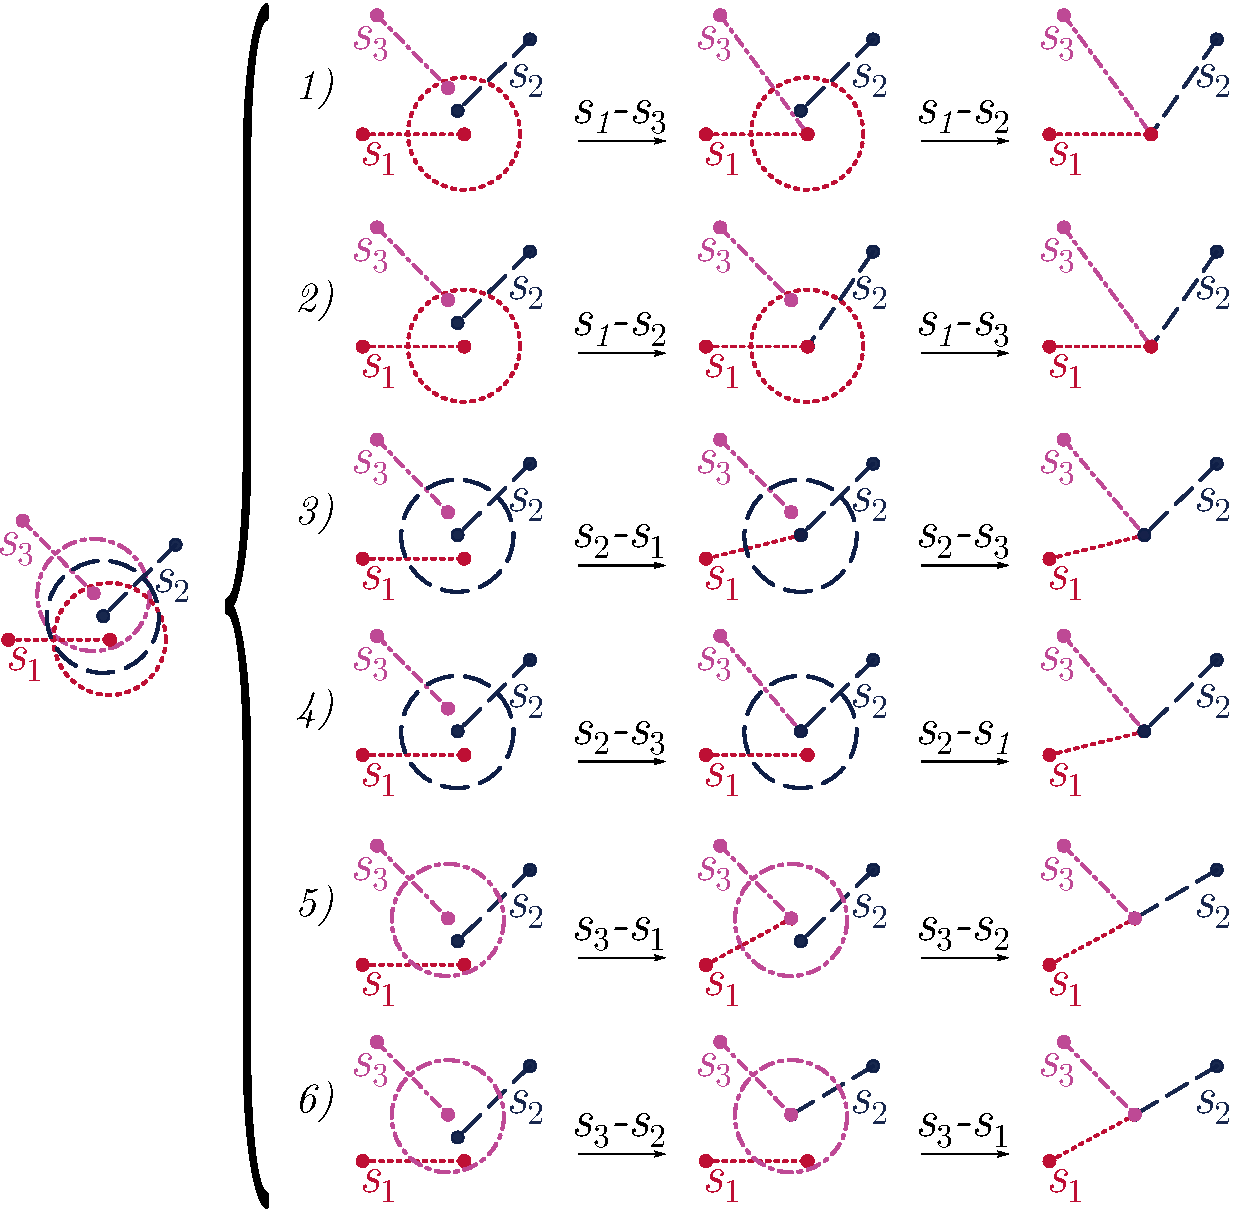
\includegraphics[width=0.5\linewidth]{collisionDist.pdf}
    \caption[Dislocation segments inside different collision radii.]{Multiple dislocation segments inside the same collision radius.}
    \label{f:collisionRadius}
\end{figure}

The actual algorithm is more sophisticated because it accounts for both complete segments and finds the two points along them with the minimum distance between each other. But the problem was that as soon as a viable collision was found, the function returned. So in a scenario like \cref{f:collisionRadius}, if the code were looking for a collision on $s_1$ and it came across $s_3$ first it would flag that as the collision disregarding the fact that not only was $s_2$ closer, but $s_2$ and $s_3$ are also closer. The same fix had to be applied to hinge collisions.

Despite the fact that checking all possible collisions for the minimum distance is a more expensive task, it results in faster simulations because the resulting structures are guaranteed to either produce the shortest segments, which can be cleaned up by remeshing, or the highest energy structures which can be cleaned up by separation. Otherwise the structures often end up in a no-man's land which is energetically unfavourable to separate, or cannot be remeshed; leading to an accumulation of highly immobile, highly energetic structures that cause more and more collisions as simulations advance and create sharp stress gradients that cause the timestep to drop significantly, and preventing simulations from advancing very much after hitting a wall.

\section{Non-commutativity of topological changes}\label{s:nonCommutativity}

For a given iteration the time-evolution of the network used to be performed before any topological changes. This was very sub-optimal for a couple of reasons.

The fundamental reason is that by doing so, the time evolution erroneously accounts for complex structures that should have dissipated into lower energey ones as per the quasi-static principle our model is based on. In other words, high energy structures in the network mean large stress gradients. These break the assumption that a node and its neighbours experience similar conditions. These locality assumptions lead to \label{eq:nodeVel}, which is what all our mobility laws based on.

The practical reason is that by leaving these structures around when they should have been removed, the computational complexity increases by virtue of having more nodes and segments that would otherwise not be there.

Moreover, the order in which topological changes were carried out was also very sub-optimal. It used to be the case that separation, collision and remeshing were performed in that order; and collision only detected a single event.

The first step was to ensure all collisions that needed to be performed in a single step were being performed. Unfortunately this quickly revealed the reason why the original version only accounted for a single collision at any given step. It made the terrifyingly-poorly-scaling separation have to separate more high energy structures every time.

The role of separation is to take high energy, highly connected structures and break them apart into lower energy, lower connection ones. Separation is a very poorly scaling operation by itself $\mathcal{O}\left(\sum\limits_{i}\sum\limits_{j=2}^{\left\lfloor C_i/2 \right\rfloor} \dfrac{C_i!}{(C_i-j)! j!}\right)$. Where the sum over $i$ is done over the nodes with more connections than is allowed; $C_i$ is the number of connections for node $i$; and $j$ is the number connections $C_i$ connections can be split into. Mirror symmetries where $2j = C_i$ half the number of possible splitting configurations for that case, but at best this puts the lower bound at approximately Sterling's factorial formula $N! = \mathcal{O}(N\log{N})$. All of these configurations must be generated, which is an $\mathcal{O}(M)$ operation where $M$ are the number of nodes to be added. Unfortunately, this is a relatively expensive operation because the code dynamically expands the relevant arrays. The nodal velocities and segment forces must be calcualted for every configuration. Whichever configuration represents the and highest energy dissipation is picked as the final configuration. Locality is assumed, so only the forces and mobilities of the segments directly involved are calculated. It is therefore extremely important that the number of separations be kept to a minimum.

The solution was as simple as calling separation after resolving a single collision. This, together with the fixes made to the collision detection, ensured only minimal energy structures were used for subsequent iterations of the collision-separation loop. It also and kept the number of possible separations low.

The final pieces of the puzzle were ensuring the network is as clean as possible before running it through the collision-separation loop. This means remeshing the network before to eliminate segments and hinges that need to be remeshed anyway and would only cause problems. And remeshing it after to ensure the next iteration has the cleanest possible network to work with.

\section{Conclusions}

These solved many of the issues with higher densities %keep writing.
\savearabiccounter
%1417